\documentclass{article}
\usepackage{listings}
\usepackage{xcolor}
\usepackage{graphicx} % Pacote para inclusão de imagens

\definecolor{backcolour}{rgb}{0.95,0.95,0.92}

\lstdefinestyle{mystyle}{
    backgroundcolor=\color{backcolour},   
    commentstyle=\color{OliveGreen},
    keywordstyle=\color{olive},
    numberstyle=\tiny\color{codegray},
    stringstyle=\color{codepurple},
    basicstyle=\ttfamily\footnotesize,
    breakatwhitespace=false,         
    breaklines=true,                 
    captionpos=b,                    
    keepspaces=true,                 
    numbers=left,                    
    numbersep=5pt,                  
    showspaces=false,                
    showstringspaces=false,
    showtabs=false,                  
    tabsize=2
}



\begin{document}
\huge{\sffamily \color{blue}Resolução}
\lstset{style=mystyle}
\lstinputlisting[language=R]{files/ex.R}

\huge{\sffamily \color{blue}Gráfico}


\begin{figure}[h] % Inicia o ambiente figure com a opção [h] para indicar que a imagem deve ser posicionada aqui (opcional)
    \centering % Centraliza a imagem
    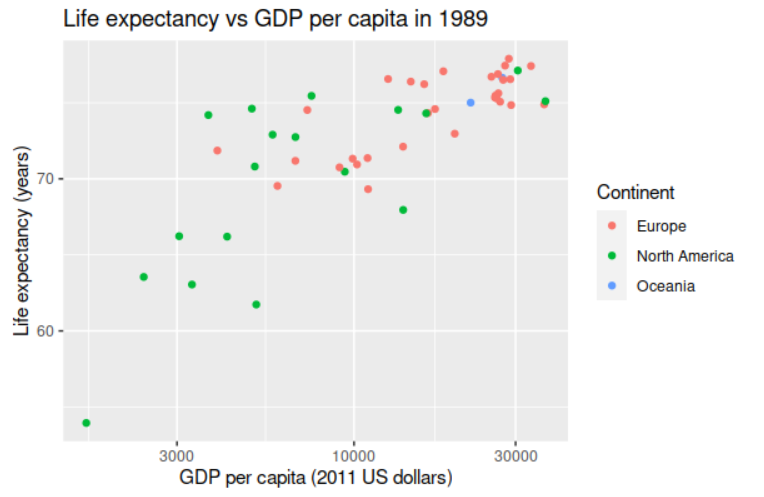
\includegraphics[width=1\textwidth]{files/graph.png} % Inclui a imagem "graph.jpg" com 50% da largura do texto
    \caption{Gráfico} % Adiciona uma legenda para a figura
    \label{fig:graph} % Adiciona uma etiqueta para referência cruzada
\end{figure}

\end{document}
